\documentclass[12pt, a4paper, UTF8]{article}
\usepackage{tikz}
\usetikzlibrary{arrows.meta, positioning, fit}

% 必需宏包
\usepackage[left=2cm,right=2cm,top=2.5cm,bottom=2.5cm]{geometry}
\usepackage{graphicx}
\usepackage{ctex}
\usepackage{fancyhdr}
\usepackage{titlesec}
\usepackage{titletoc}
\usepackage{caption}
\usepackage{footmisc} % 脚注格式
\usepackage{enumitem} % 启用自定义列表参数
\usepackage{amsmath}
\usepackage{array}
\usepackage{setspace}

% 英文字体
\usepackage{fontspec}
\setmainfont{Times New Roman}
\setsansfont{Arial}
\setmonofont{Consolas}

% 附件 3 要求图表按章编号为“图 m-n”“表 m-n”；本文以 article 的 section 对应“章”。
\counterwithin{figure}{section}
\counterwithin{table}{section}
\renewcommand{\thefigure}{\thesection-\arabic{figure}}
\renewcommand{\thetable}{\thesection-\arabic{table}}


% 页眉页脚（篇眉：宋体五号，居中）
\pagestyle{fancy}
\fancyhf{}
\fancyhead[C]{\songti\zihao{5} 第二十一届中国研究生电子设计竞赛\\多MCU协同光储一体化数字电源系统}
\fancyfoot[C]{\thepage}
\setlength{\headheight}{28pt}

% 标题格式（严格对齐规范）
\titleformat{\section}
  {\centering\heiti\zihao{-2}} % 黑体小二号（18pt），居中
  {第\thesection 章}
  {1em}{}

\titleformat{\subsection}
  {\heiti\zihao{-3}} % 黑体小三号（14pt），顶头
  {\thesubsection}
  {1em}{}

\titleformat{\subsubsection}
  {\heiti\zihao{-4}} % 黑体小四号（12pt），顶头
  {\thesubsubsection}
  {1em}{}


% 脚注格式：宋体小五号 + 全文连续编号 + ①②③样式
\usepackage{pifont}
\renewcommand{\thefootnote}{\ding{\numexpr171+\value{footnote}}} % ①②③...
\renewcommand{\footnotelayout}{\songti\zihao{-5}} % 宋体小五号

% 目录格式（按之前要求）
\renewcommand{\contentsname}{}
\titlecontents{section}
  [0em]
  {\heiti\zihao{4}} % 四号黑体
  {第\thecontentslabel\ 章\ }
  {}
  {\titlerule*[0.8pc]{.}\contentspage}
\titlecontents{subsection}
  [2em]
  {\songti\zihao{-4}} % 小四宋体
  {\thecontentslabel\ }
  {}
  {\titlerule*[0.8pc]{.}\contentspage}
\titlecontents{subsubsection}
  [4em]
  {\songti\zihao{-4}} % 小四宋体
  {\thecontentslabel\ }
  {}
  {\titlerule*[0.8pc]{.}\contentspage}

% 链接无框
\usepackage[hidelinks]{hyperref}

% 附件 3：正文段落与标题固定行距 20 pt（Word「固定值 20 磅」；article 12 pt 下 \normalsize
% 默认行距约 14.5 pt，故 \setstretch{20/14.5}）。若标题需绝对 20 pt 行距，再在 \titleformat 内单独设。
\AtBeginDocument{\setstretch{1.379310}}

\newcommand{\todo}[1]{\textbf{TODO：#1}}

\begin{document}

\begin{titlepage}
\centering
\vspace*{1cm}
{\zihao{1}\heiti 第二十一届中国研究生电子设计竞赛\par}
\vspace{0.5cm}
{\zihao{1}\heiti 技术论文\par}
\vspace{1.5cm}
{\zihao{-2}\heiti 论文题目：多 MCU 协同光储一体化数字电源系统\par}
\vspace{0.3cm}
{
\setlength{\baselineskip}{18pt}
\zihao{-2}\sffamily
Integrated PV-Storage Digital Power System\\ with Multi-MCU Coordination\par
}
\vspace{3cm}
\begin{flushleft}
\hspace*{4cm}
\begin{minipage}{0.6\textwidth}
\zihao{-3}\heiti
参赛单位：西安电子科技大学\\[0.4cm]
队伍名称：传奇要饭王\\[0.4cm]
指导老师：韩卫华、杨如森\\[0.4cm]
参赛队员：江达伟、卢沐阳、曹张振\\[0.4cm]
完成时间：2026年6月20日
\end{minipage}
\end{flushleft}
\end{titlepage}


% ================= 前置部分无页码 =================
\pagestyle{empty}
% !TeX root = ../technical_paper.tex
\clearpage
\section*{摘要}

针对家庭储能、分布式光伏和离网备用供电对高效率、高可靠性和智能化管理的需求，本文设计并实现了一套多 MCU 协同光储一体化数字电源系统。系统面向小型家庭能源场景，集成光伏输入、储能电池管理、直流母线稳压、单相交流输出和无线监控等功能，形成从新能源接入到交流负载供电的完整闭环。

系统采用非隔离三端口功率变换架构，将光伏端口、储能端口和直流母线端口统一到前级功率变换器中，并通过后级交流变换单元输出 220 V/50 Hz 单相交流电。控制系统由 GD32G553、GD32C113 和 GD32VW553 三颗 MCU 协同完成：GD32G553 负责主功率变换、MPPT、母线稳压和交流控制；GD32C113 负责电池电压、电流、温度采样以及 SOC 估算、均衡和保护；GD32VW553 负责无线联网、参数配置、运行日志和告警信息管理。通过功能解耦与通信协同，系统兼顾功率控制实时性、电池安全性和用户侧可观测性。

本文重点阐述系统难点与创新、总体方案、主功率电路、控制电路、软件流程及测试验证方法。系统实现了光伏 MPPT 跟踪、光储多模态能量调度、离网工况下电压/频率稳定控制、SOC 估算和多级安全保护。初步设计表明，该方案具备结构紧凑、控制灵活、扩展性好和工程落地成本较低等特点，可为户用光储一体化设备和小型备用电源提供一种基于国产 MCU 的数字控制实现路径。

\vspace{1em}
\noindent\textbf{关键词：} 光储一体化；三端口变换器；多 MCU 协同；GD32；MPPT；BMS

\clearpage
\section*{Abstract}

To meet the requirements of household energy storage, distributed photovoltaic generation, and off-grid backup power supply, this paper presents an integrated photovoltaic-storage digital power system based on multi-MCU coordination. The system integrates photovoltaic input, battery management, DC bus regulation, single-phase AC output, and wireless monitoring, providing a complete energy conversion path from renewable energy input to AC load supply.

The proposed system adopts a non-isolated three-port power conversion architecture. The photovoltaic port, battery port, and DC bus port are coordinated by the front-stage converter, while the rear-stage AC converter generates 220 V/50 Hz single-phase AC output. Three GD32 microcontrollers are used for task decomposition and cooperative control. The GD32G553 handles main power conversion, MPPT, DC bus regulation, and AC output control. The GD32C113 performs battery voltage, current, and temperature sampling, SOC estimation, balancing, and protection. The GD32VW553 provides wireless networking, parameter configuration, operation logging, and alarm management. With this architecture, the system balances real-time power control, battery safety, and remote observability.

This paper describes the technical challenges, innovation points, system architecture, power circuit, control circuit, software flow, and verification plan. The system supports photovoltaic MPPT tracking, multi-mode energy scheduling, off-grid voltage and frequency regulation, SOC estimation, and multi-level protection. The design provides a compact, flexible, and low-cost digital control solution for residential photovoltaic-storage integrated equipment based on domestic MCU devices.

\vspace{1em}
\noindent\textbf{Keywords:} photovoltaic-storage integration; three-port converter; multi-MCU coordination; GD32; MPPT; BMS



% ================= 目录 =================
\clearpage
\begin{center}
\heiti\zihao{3} 目\quad 录
\end{center}
%\vspace{1em}
\tableofcontents

% ================= 正文开始 =================
\clearpage
\pagestyle{fancy}
\pagenumbering{arabic}
\setcounter{page}{1}

\section{作品难点与创新}

本作品面向家庭储能与分布式光伏离网供电场景，提出一种基于 GD32 系列 MCU 的光储逆变一体化能源电力系统。系统由光伏输入模块、储能电池及 BMS 模块、前级三端口功率变换器、后级单相逆变模块和无线监控模块构成，能够完成光伏能量接入、电池安全管理、交流输出供电和远程监测控制。

系统采用 GD32G553、GD32C113 和 GD32VW553 三颗 MCU 分工协作。其中，GD32G553 作为主功率控制器，负责光伏输入功率变换、储能充放电控制、直流母线调节和逆变输出控制；GD32C113 作为电池管理控制器，负责电芯采样、均衡、SOC 估算和故障保护；GD32VW553 作为联网控制器，负责无线通信、参数配置、运行日志和告警信息管理。该架构既保证底层功率环路的实时性，又提升了系统安全性和用户侧交互能力。

\subsection{应用场景与作品定位}

户用光储系统通常需要同时满足光伏高效利用、储能安全运行、离网交流供电和远程运维管理等需求。传统分立式方案往往由光伏控制器、充电器、逆变器和监控模块独立构成，系统体积较大、通信链路复杂、能量调度不够统一。本作品将光伏输入、储能电池和逆变输出统一纳入数字电源控制框架，重点解决小功率家庭备用供电场景下的集成化、智能化和国产化控制实现问题。

本系统的目标不是单一变换器验证，而是完成从电源硬件、控制算法、电池保护到无线监控的整机方案。论文后续章节将围绕系统架构、主功率电路、控制策略、保护机制和测试验证展开。

\subsection{难点分析}

实现一个光伏、储能、逆变一体化的微型数字电源系统，主要面临以下难题：

\begin{enumerate}[label=\arabic*、, leftmargin=*, itemsep=0.8ex, parsep=0pt, topsep=0.5ex]
  \item 小型化趋势与直流母线高压需求之间存在矛盾。为实现兼具体积和功率密度的三端口功率变换器，非隔离拓扑结构成为优选方案。然而，将低压光伏与电池端口提升至逆变所需直流母线，会使变换器在高电压增益条件下运行，对开关器件、电感设计和控制稳定性提出更高要求。
  \item 多端口强耦合与协调控制难。光伏、储能和直流母线三者之间存在能量耦合，不同工况下需要同时满足光伏高效利用、母线稳定、电池安全和负载供电，控制目标相互约束，容易出现能量冲突、母线波动或模式误判。
  \item 多模式平滑切换难度大。系统需在光伏优先、光伏充电、电池放电、混合供电、欠压保护和过载保护等模式间切换，不同模式的控制目标和限值条件差异较大，若切换逻辑处理不当，可能引发电压跌落、电流冲击和逆变输出畸变。
  \item GD32 数字控制实时性要求高。三端口变换和单相逆变需要多路电压、电流和功率同步采样，同时完成 PWM 更新、多环路闭环计算和故障中断处理，对 GD32G553 的外设配置、中断优先级和算法执行效率提出较高要求。
  \item BMS 与主功率系统协同难。电池 SOC 估算、均衡和保护需要与三端口充放电策略深度联动，既要保证电池不过充、不过放和不过温，又不能牺牲母线动态响应和负载供电连续性。
  \item 逆变输出与直流母线动态耦合明显。交流负载突变会直接扰动直流母线，前级三端口调节与后级逆变稳压之间必须协调设计，才能兼顾母线稳定、输出电压质量、动态响应和带载能力。
  \item 多 MCU 协同与无线监控实时性需要平衡。GD32G553、GD32C113 和 GD32VW553 分工协作，需要设计可靠通信协议和故障联动逻辑；无线监控数据上传和参数下发不能干扰底层功率控制实时性。
\end{enumerate}

\subsection{创新点分析}

针对以上难点，本团队从拓扑集成、控制架构、能量调度和系统安全四个层面进行设计，形成以下创新点：

\begin{enumerate}[label=\arabic*、, leftmargin=*, itemsep=0.8ex, parsep=0pt, topsep=0.5ex]
  \item 非隔离三端口光储变换架构。系统将光伏端口、储能端口和直流母线端口统一到前级功率变换器中，相比传统分立式光伏控制器加电池充电器方案，减少能量变换级数和控制接口，有利于提升整机集成度和响应速度。
  \item 多 MCU 协同控制架构。构建 GD32G553、GD32C113、GD32VW553 三芯片协同架构，分别承担主功率控制、电池安全管理和无线监控任务，实现实时控制、安全保护和通信交互解耦，充分发挥 GD32 系列 MCU 在数字电源控制、BMS 管理和无线互联方面的综合能力。
  \item 光储协同多模态能量调度策略。提出以光伏优先利用、母线稳定和电池安全为约束的能量调度逻辑，根据光伏功率、负载功率、电池 SOC 和故障状态自动选择工作模式，实现储能自适应充放电和离网稳压运行。
  \item 面向工程应用的分层保护机制。系统在硬件比较、MCU 快速中断、BMS 状态机和无线告警层面设置多级保护，对过压、欠压、过流、过温、通信异常和电池异常进行分层处理，提高整机运行可靠性。
  \item 可扩展远程监控与参数配置。基于 GD32VW553 实现无线联网，将运行数据、故障日志和关键参数上传至上位机或移动端，为后续远程运维、数据分析和算法在线优化提供接口。
\end{enumerate}

\clearpage
% !TeX root = ../technical_paper.tex


\section{方案论证与设计}

\subsection{总体方案}

本作品面向户用储能、离网备用供电与远程状态监测等应用场景，采用 GD32G553 主控、GD32C113 BMS 和 GD32VW553 无线模块构成的三节点协同架构。系统设计的重点不是将所有功能压缩到单一控制器内，而是通过明确分工、统一接口与状态机管理，实现采样、保护、转发、监控和参数交互等功能的协同运行。其总体设计遵循“本地安全优先、控制与监控解耦、接口统一、状态可追踪”的原则。

其中，GD32G553 主控负责系统调度、BMS 数据接收与转发、HRTIMER PWM 输出以及基础采样管理；GD32C113 BMS 负责电池测量、保护判断、FET 策略、均衡控制和 SOC 估算；GD32VW553 负责无线通信、页面展示、参数配置和告警信息管理。三者之间通过 CAN FD 与 UART 等链路连接，构成从电池侧状态采集到远程监控展示的完整闭环。

从工程实现角度看，该方案的优点在于：一方面，主控侧可以专注于实时性较强的控制与转发任务；另一方面，BMS 侧可以专注于电池安全与状态管理；无线侧则承担低实时性的交互任务。这样既避免了单 MCU 同时承担控制、保护和通信而导致的软件耦合过深，也降低了调试和后期扩展的复杂度。

\begin{figure}[htbp]
  \centering
  \resizebox{\linewidth}{!}{
  \begin{tikzpicture}[
    font=\small,
    block/.style={draw, rounded corners=2pt, align=center, minimum width=3.1cm, minimum height=1.0cm},
    bigblock/.style={draw, rounded corners=2pt, align=center, minimum width=4.2cm, minimum height=1.6cm},
    line/.style={-Latex, thick},
    dline/.style={-Latex, thick, dashed}
  ]

  % Power ports
  \node[block] (pv) {光伏输入端\\PV};
  \node[block, right=2.8cm of pv] (power) {三端口功率板};
  \node[block, right=2.8cm of power] (out) {输出端 / 负载\\VOUT};

  % Internal power board functions
  \node[block, above=1.4cm of power] (driver) {隔离驱动与保护\\UCC21540\\OC\_FAULT};
  \node[block, below=1.1cm of power] (sample) {采样调理\\V\_PV / I\_PV\\V\_OUT / I\_OUT\\TEMP};

  % Controller
  \node[bigblock, below=2.4cm of pv] (g553) {GD32G553 主控制板\\系统调度 / ADC 采样\\HRTIMER PWM / 故障输入\\CAN / UART};

  % Battery below controller
  \node[block, below=1.4cm of g553] (bat) {16S 磷酸铁锂电池组\\BAT};

  % BMS
  \node[bigblock, right=3.8cm of bat] (bms) {GD32C113 BMS 板\\GD30BM2016 AFE\\单体采样 / 电流检测\\均衡 / FET 保护 / SOC};

  % WiFi and host
  \node[bigblock, right=2.5cm of sample] (wifi) {GD32VW553 无线模块\\WiFi 通信\\数据转发 / 参数交互};
  \node[block, right=2.5cm of wifi] (app) {上位机 / App\\状态显示\\模式切换\\故障告警};

  % Power flow
  \draw[line] (pv) -- node[above]{能量输入} (power);
  \draw[line] (power) -- node[above]{稳压输出} (out);

  % Control and sampling
  \draw[line] (g553.north)  ++(-2,0)|- node[pos=0.25, left]{PWM 驱动信号} (driver.west);
  \draw[line] (driver.south) -- node[right]{栅极驱动} (power.north);
  \draw[line] (sample.west) -- node[pos=0.6, above=0.4cm]{ADC 反馈} (g553.east);
  \draw[dline] (power.south) -- (sample.north);

  % BMS links
  \draw[line] (bat.east) -- node[below]{单体电压 / 电流 / 温度} (bms.west);
  \draw[line] (bms.north west) -- node[pos=0.1, above=0.38cm]{CAN FD 遥测 / 保护状态} (g553.south east);

  % Wireless links
  \draw[line] (g553.east) ++(0,-0.45) -| node[pos=0.4,above]{UART 数据帧} (wifi.south);
  \draw[line] (wifi.east) -- node[above]{WiFi} (app.west);
  \draw[dline] (app.south) -- ++(0,-0.45) -| node[pos=0.25, below]{参数配置 / 模式命令} (wifi.south);

  \end{tikzpicture}
  }
  \caption{系统总体架构示意图}
  \label{fig:system_architecture}
\end{figure}


系统的核心设计思想是将强实时任务与弱实时任务分离。功率变换闭环、PWM 更新和快速保护由 GD32G553 就近完成；电池状态估算、均衡和电池侧保护由 GD32C113 独立完成；无线通信、数据记录和人机交互由 GD32VW553 承担。通过任务分层，系统避免了无线通信和日志处理对功率控制中断的干扰。


\subsection{主要参数与系统规格}

表 \ref{tab:spec} 给出了本系统的目标规格。

\begin{table}[htbp]
  \centering
  \caption{系统目标规格}
  \label{tab:spec}
  \begin{tabular}{|p{0.28\linewidth}|p{0.26\linewidth}|p{0.34\linewidth}|}
    \hline
    项目 & 设计目标 & 说明 \\
    \hline
    光伏输入电压 & 约 36 V 等级 & 面向低压光伏输入场景，便于与实验电源和光伏模拟源进行联调 \\
    \hline
    储能电池电压 & 约 48 V 等级 & 单体标称电压 3.2 V，满充电压约 58.4 V，放电截止附近约 40 V \\
    \hline
    直流母线电压 & 满足 220 V/50 Hz 交流输出需求 & 为后级 220 V/50 Hz 单相交流输出预留直流母线电压裕量 \\
    \hline
    交流输出 & 220 V/50 Hz 单相交流 & 离网备用供电场景 \\
    \hline
    额定功率 & 约 200 W 等级 & 依据器件、电感和散热能力确定 \\
    \hline
    控制平台 & GD32G553、GD32C113、GD32VW553 & 主功率控制、BMS、无线监控分工 \\
    \hline
    保护功能 & 过压、欠压、过流、过温、通信异常 & 硬件保护与软件状态机结合 \\
    \hline
  \end{tabular}
\end{table}

\subsection{方案选择与论证}

本作品采用多 MCU 协同方案，主要基于以下考虑。

\begin{enumerate}[label=\arabic*、, leftmargin=*, itemsep=0.8ex, parsep=0pt, topsep=0.5ex]
  \item \textbf{实时控制与远程交互的实时性要求不同。}  
  主控和 BMS 的采样、判断、保护动作需要较高实时性，而网页展示、参数配置和日志传输允许较低刷新频率。若将两类任务集中在单一控制器内，容易造成中断拥塞、控制周期抖动和异常响应延迟。

  \item \textbf{电池安全控制需要独立闭环。}  
  BMS 不应仅作为主控的一个附属采样模块，而应独立完成测量、保护、均衡和 FET 策略。这样在发生过压、欠压、过温、采样异常或通信异常时，BMS 可立即执行降级和关断策略，保证电池安全优先。

  \item \textbf{监控系统不应干扰底层控制。}  
  无线通信、数据展示和参数配置本质上属于非实时任务，如果和底层保护逻辑耦合过紧，一旦网络阻塞或页面刷新异常，就可能影响核心控制链路。因此，需要把监控链路从控制链路中剥离出来。

  \item \textbf{模块化设计有利于后续扩展。}  
  采用主控、BMS、无线模块分层设计后，后续若要增加新的采样项、告警类型或页面字段，只需扩展对应模块即可，不必重构整个系统。
\end{enumerate}
因此，本作品最终选择“主控负责调度与转发、BMS 负责安全与状态、无线模块负责展示与交互”的系统分工方式，并通过统一数据格式与状态编码将各模块连接起来。
\subsection{控制芯片分工}

\subsubsection{GD32G553 与主功率控制}

GD32G553 主控工程采用四层解耦架构，将系统划分为 APP 层、Middleware 层、Protocol 层和 HAL 层。该结构的核心思想是让应用逻辑、数据管理、协议处理和底层驱动相互隔离，从而提升代码清晰度和可移植性。

在 APP 层，系统通过统一调度器组织各模块运行，包括 BMS 数据转发、心跳帧输出和 HRTIMER PWM 任务等；在 Middleware 层，采用发布/订阅式数据总线组织系统内部数据流，使数据生产者与消费者解耦；在 Protocol 层，完成 CAN FD 帧解析与 UART AA55 帧封装；在 HAL 层，则对 CAN、UART、HRTIMER 等外设进行统一抽象，使上层逻辑不直接依赖具体硬件实现。

主控侧的核心任务主要包括以下几个方面：其一，通过 CAN FD 接收 BMS 遥测数据，并解析电池电压、电流、温度、SOC、均衡状态和故障标志；其二，将上述信息通过 UART 转发给 Wi-Fi 模块，供页面显示和远程交互使用；其三，输出 HRTIMER PWM，为功率控制链路提供基础接口；其四，对基础 ADC 采样数据进行校准和换算，以支持系统联调和物理量显示。该设计使主控既能承担系统级组织任务，又不会陷入低层驱动细节。

\begin{figure}[htbp]
  \centering
  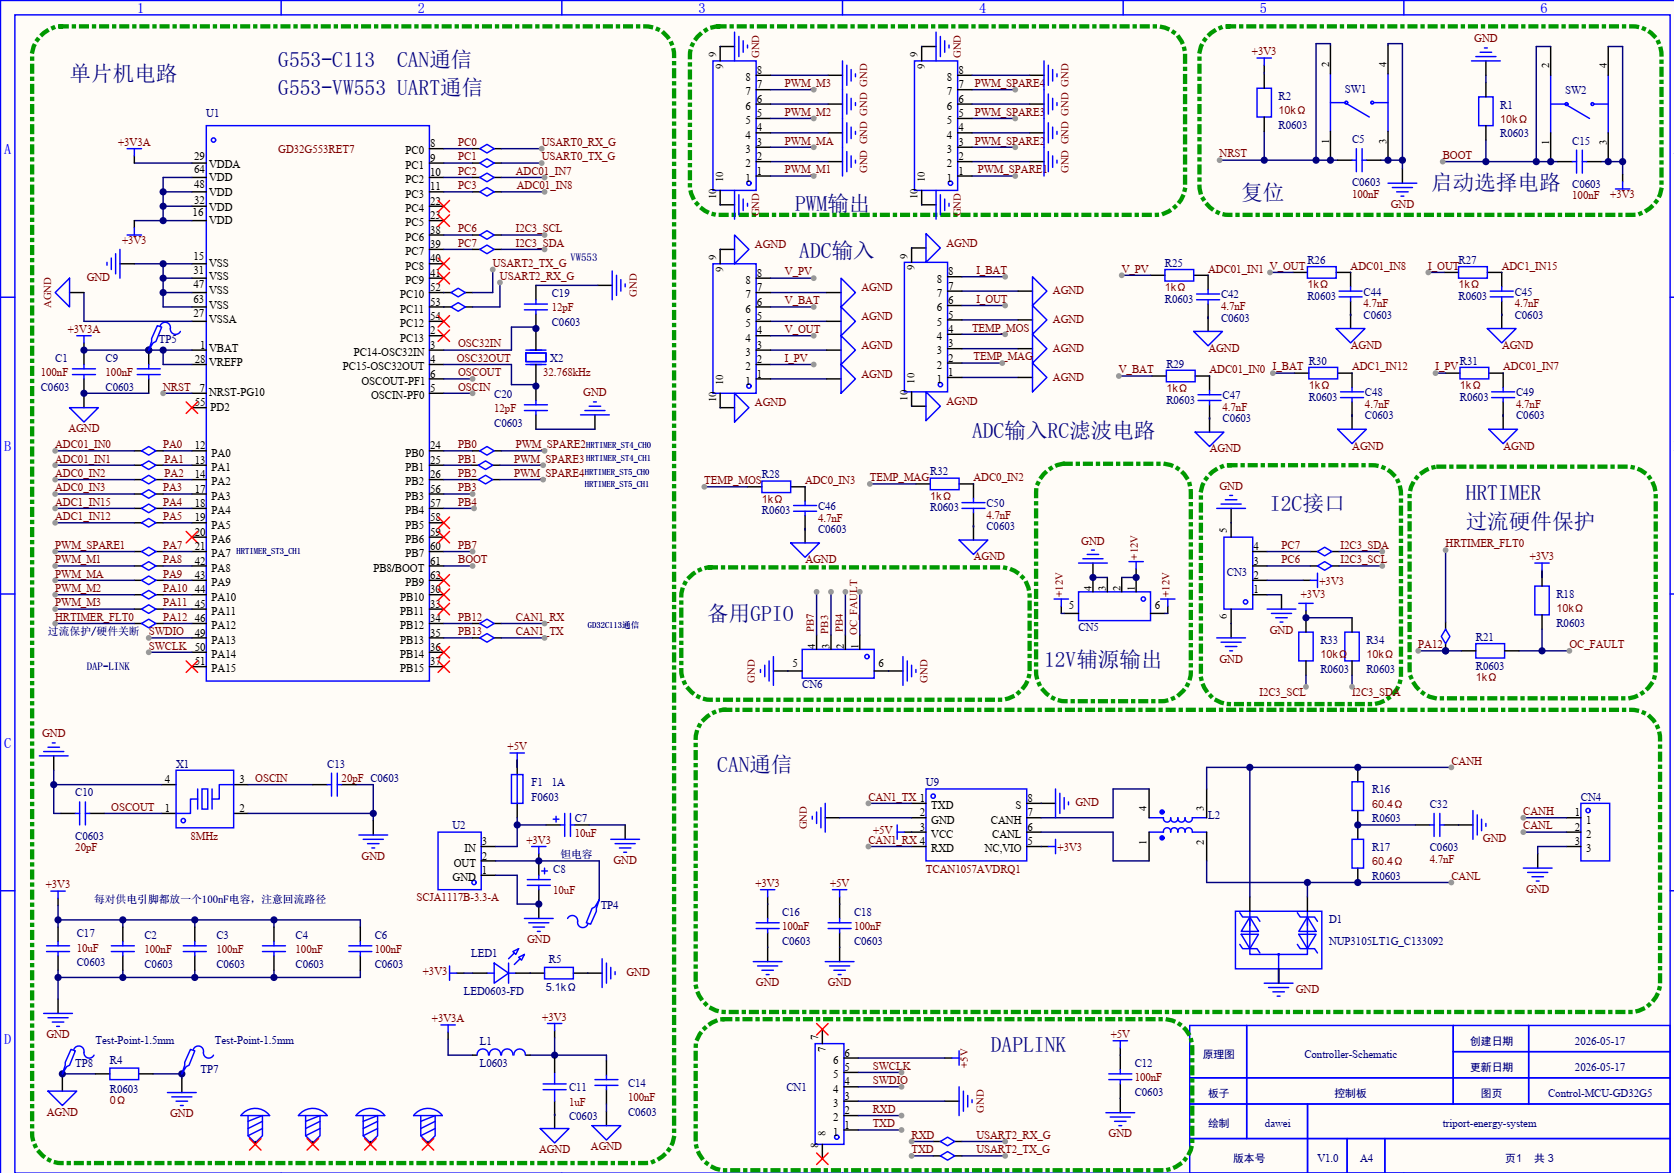
\includegraphics[width=0.8\textwidth]{images/主控板原理图1.png}
  \caption{主功率控制原理图1}
  \label{fig:system_architecture}
\end{figure}

\begin{figure}[htbp]
  \centering
  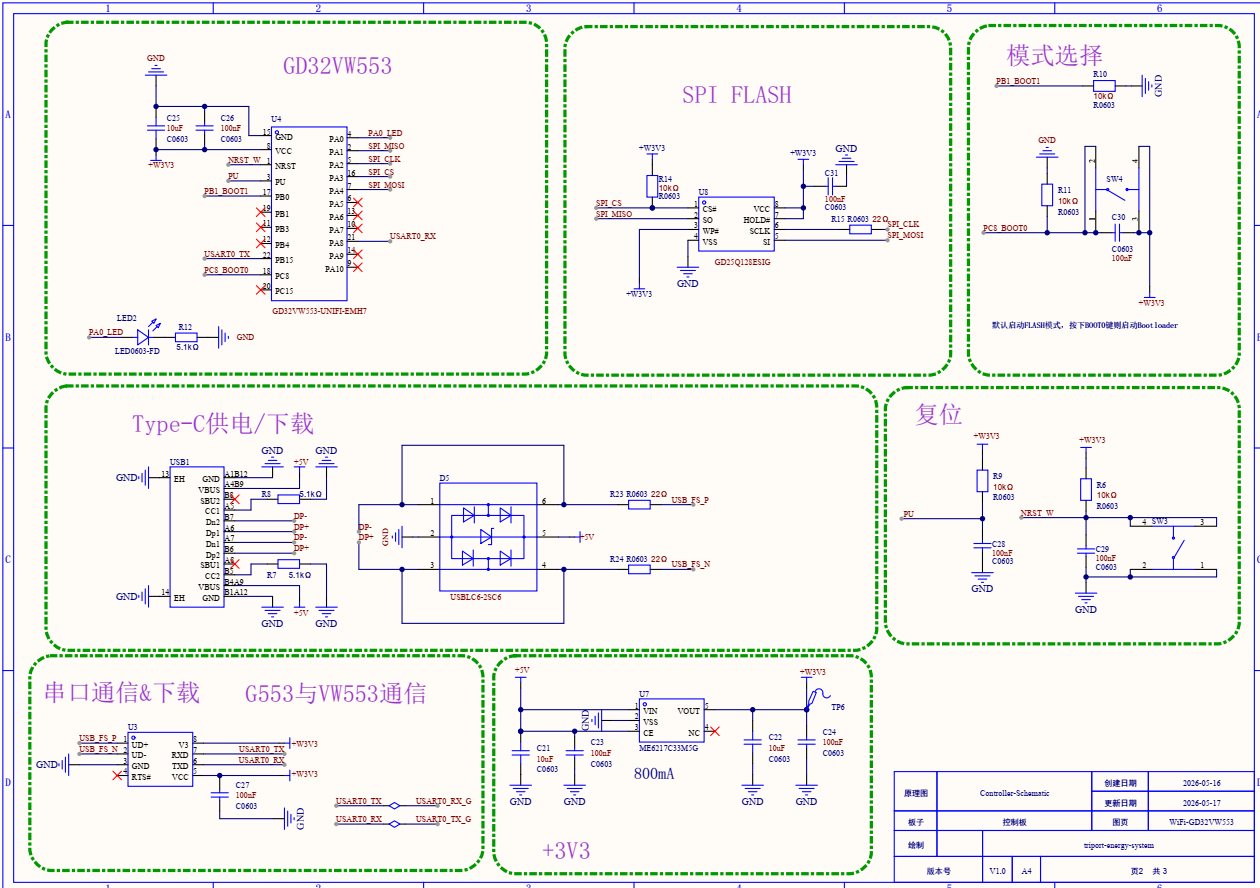
\includegraphics[width=0.8\textwidth]{images/主控板原理图2.png}
  \caption{主功率控制原理图2}
  \label{fig:system_architecture}
\end{figure}

\begin{figure}[htbp]
  \centering
  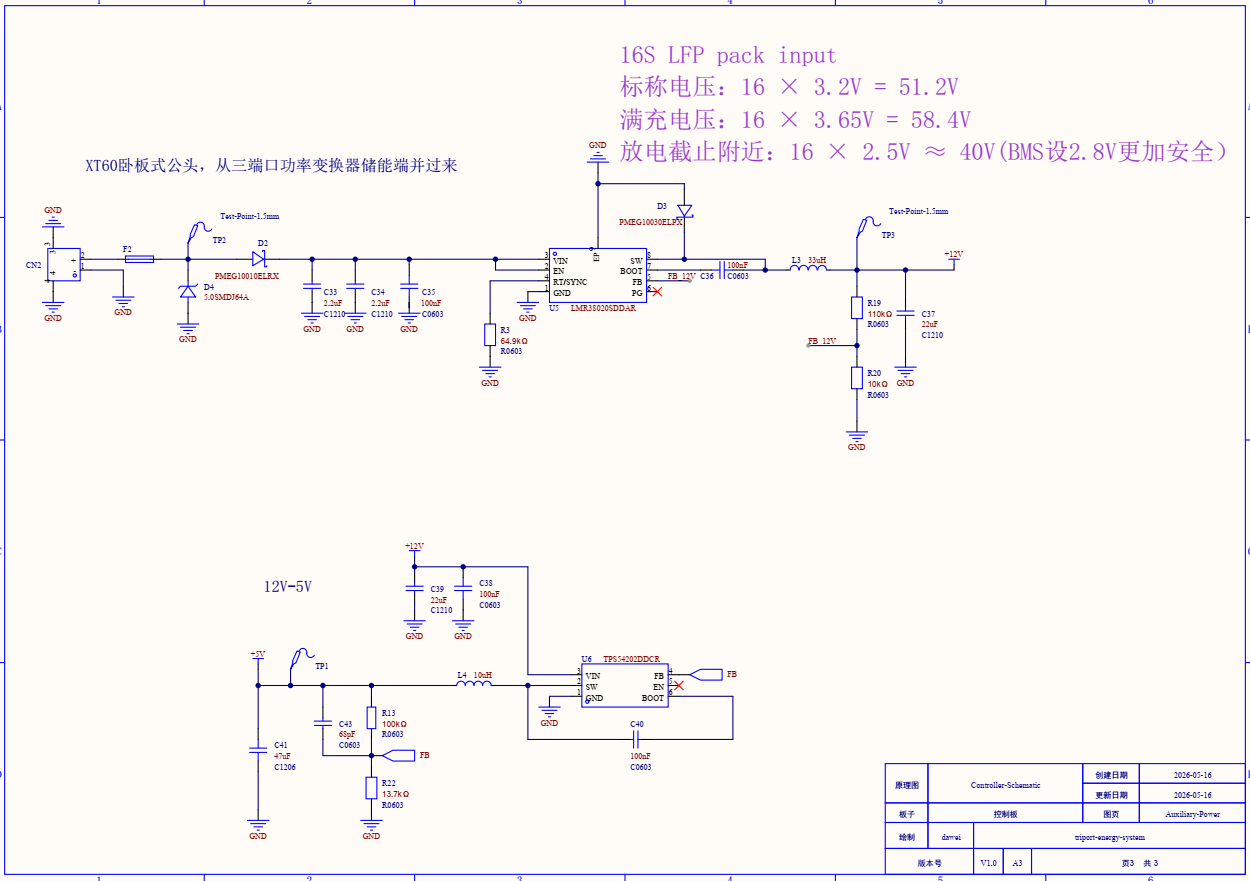
\includegraphics[width=0.8\textwidth]{images/主控板原理图3.png}
  \caption{主功率控制原理图3}
  \label{fig:system_architecture}
\end{figure}

\subsubsection{GD32C113 与 BMS}

GD32C113 BMS 工程采用产品态机和功能模块分层的方式组织软件。其核心模块包括测量、保护、FET、均衡和 SOC 五部分：测量模块负责 AFE 唤醒、配置和数据读取；保护模块负责安全状态与故障判断；FET 模块负责充放电通路控制；均衡模块负责单体均衡请求和执行；SOC 模块负责静置 OCV 估算与库仑计累计。在系统运行过程中，这些模块并不是孤立执行，而是按照统一的状态机顺序进行协同。

BMS 的产品状态机主要包含 INIT FAIL、RUN 和 DEGRADED 三种状态。系统上电后，首先执行板级初始化和 AFE 最小唤醒，然后关闭 FET 通路并清除均衡，再进入完整配置流程，包括 16S 配置、CCGain 设置以及保护项装载。只有当首次测量有效、无严重故障且电芯状态正常时，系统才进入 RUN 状态。若运行过程中出现读取失败、保护触发、FET 应用失

败或严重安全异常，则立即进入 DEGRADED 状态，执行均衡抑制和 FET 全关断，待故障恢复后再返回正常运行。

该设计的关键价值在于将电池安全放在最高优先级。与简单的“采样后直接上报”不同，BMS 在本作品中承担的是一个完整的安全控制节点职责：既要保证测量准确，又要保证故障可追踪、保护可锁存、状态可回显。通过这种方式，BMS 不再只是被动数据源，而成为系统安全闭环中的核心一环。


\subsubsection{GD32VW553 与无线监控}

GD32VW553 主要承担系统的无线通信、人机交互和数据上报功能，是整套平台的远程监控入口。其工作方式是接收主控制器转发的运行状态、关键测量值和告警信息，并对数据进行协议解析、缓存与打包后发送至无线终端或上位机界面。与此同时，GD32VW553 还可接收上位机下发的参数配置、模式切换与查询指令，并将其转换为统一的内部命令格式后转发至主控执行。  

在系统架构上，无线模块不直接参与电压、电流等快速闭环控制，而是作为信息交互层存在。这样设计能够保证主功率控制与通信显示解耦，避免网络抖动、丢包或界面卡顿对核心控制环路造成干扰。该模块的意义不仅在于提升系统可观测性，也在于增强调试效率和故障定位能力，使设备的运行状态、历史数据和异常事件能够被及时记录与追踪。  

无线监控层重点支持运行状态展示、故障告警、基础参数查询和数据记录等功能。对于后续扩展，还可以进一步增加运行日志导出、远程参数整定和维护提示等功能，从而形成较完整的远程监测与交互界面。

\subsection{三端口功率变换方案设计}

本系统主功率部分采用面向光伏输入、电池储能和负载输出的三端口功率变换方案。该方案的设计目标是在统一功率级中组织光伏端、储能端和输出端之间的能量流动关系，为后续实现光伏输入利用、电池充放电控制和输出稳压提供硬件基础。与将光伏变换、电池充放电和输出变换完全分立的方案相比，三端口结构能够减少级联变换环节，使系统在结构紧凑性、能量调度灵活性和后续扩展能力方面具有优势。

结合功率板原理图，三端口主功率电路主要由 PV 端、BAT 端、VOUT 端、四绕组耦合电感、主功率开关器件、续流与钳位器件、采样调理电路和隔离驱动电路组成。其中，PV 端用于接入光伏输入，BAT 端用于连接储能电池，VOUT 端用于形成后级输出。四绕组耦合电感作为能量传递与端口耦合的核心器件，用于建立不同端口之间的磁耦合关系。通过调节不同开关管的导通状态和 PWM 占空比，可以为后续实现光伏到输出、光伏到电池、电池到输出等不同能量路径提供基础。

从主功率器件配置看，功率板中选用了 IRFP4668PBF、IPB073N15N5、BSC0702LS 和 GC4D05120A 等功率器件，用于构成不同端口之间的开关调制通道。功率开关由主控制板输出的 \texttt{PWM\_M1}、\texttt{PWM\_MA}、\texttt{PWM\_M2} 和 \texttt{PWM\_M3} 等信号进行控制。该设计使主控制板能够根据系统运行模式调整不同端口的能量流向，为充电、放电和输出调节等工况提供控制接口。由于三端口功率变换涉及多个端口的电压、电流和功率耦合关系，其控制复杂度高于普通单输入单输出变换器，因此在方案设计阶段需要同步考虑功率拓扑、驱动隔离、采样反馈和故障保护。

\subsection{三端口功率板采样与驱动设计}

为满足后续闭环控制和保护判断需求，功率板针对光伏端、输出端和关键器件温度设计了采样接口。采样信号包括光伏输入电压 \texttt{V\_PV}、输出电压 \texttt{V\_OUT}、光伏输入电流 \texttt{I\_PV}、输出电流 \texttt{I\_OUT}、MOSFET 温度 \texttt{TEMP\_MOS} 和磁性器件温度 \texttt{TEMP\_MAG}。其中，电压采样采用高阻分压和运算放大器缓冲方式，将高压侧信号转换至控制器 ADC 可采集范围；电流采样采用分流电阻配合 INA181 电流检测芯片完成信号调理；温度采样用于监测功率器件和磁性器件的热状态。

从原理图可以看出，功率板输出端按照较高电压等级进行设计，因此输出电压采样部分采用多级高阻分压，以降低单个电阻承受的电压应力。采样后端通过 OPA2188 运算放大器进行缓冲和调理，提高采样信号的稳定性和抗干扰能力。电流采样部分通过 \texttt{I\_PV+}、\texttt{I\_PV-}、\texttt{IOUT+} 和 \texttt{IOUT-} 等差分检测节点获取电流信息，再由 INA181 输出与电流成比例的电压信号。该采样链路能够为后续 MPPT、充电限流、放电限流、输出稳压和异常保护提供数据基础。

驱动部分采用 UCC21540ADWKR 隔离驱动芯片，并为各功率开关支路配置隔离电源。隔离驱动能够在控制侧和功率侧之间建立电气隔离，降低高 $dv/dt$ 开关节点对 MCU 控制信号的干扰。驱动网络中设置了栅极电阻、下拉电阻、去耦电容和关断控制信号，用于改善开关速度、抑制误导通并增强故障状态下的关断可靠性。同时，功率板预留了 \texttt{OC\_FAULT} 等故障接口，可与主控制板的 HRTIMER 故障输入配合，在出现过流或异常状态时实现快速关断。

\subsection{三端口方案仿真与板级实现}

在本阶段，三端口功率变换部分已经完成电路仿真和功率板原理图及 PCB 设计。仿真主要围绕充电、放电和端口切换等典型工况展开，重点观察各端口电压电流变化、功率器件开关状态、耦合电感电流变化以及控制量调节过程。通过仿真可以验证三端口方案在功能逻辑上的可行性，并为后续实物调试提供初始参数参考。

板级实现方面，功率板已经按照主功率回路、采样调理回路和隔离驱动回路进行功能划分。主功率区域围绕四绕组耦合电感和功率开关器件布置，采样区域负责将高压、大电流和温度信号转换为控制器可读取的低压信号，驱动区域负责接收主控制板 PWM 信号并驱动功率器件。该划分有利于降低控制信号与功率开关噪声之间的相互干扰，也便于后续分模块调试。

需要说明的是，当前三端口功率板已经完成仿真和板级设计，但实物测试仍需进一步开展。后续测试将按照由低压到高压、由开环到闭环、由单端口到多端口协同的顺序推进。首先验证隔离驱动、电源、采样和保护接口是否正常；随后在限压限流条件下测试单端口能量传递和开关波形；最后逐步开展充放电闭环、输出稳压和多模式切换测试。通过这种分阶段测试方式，可以降低功率级调试风险，并逐步验证三端口方案在实际硬件中的可行性。

综上，三端口功率变换方案是本系统后续实现光伏、储能和输出协同控制的重要基础。其设计已经覆盖主功率拓扑、采样反馈、隔离驱动和故障保护接口，并与 GD32G553 主控制板、GD32C113 BMS 板和 GD32VW553 无线监控模块形成清晰的系统连接关系。该方案为后续完成实物闭环控制、功率级性能测试和整机能量调度优化提供了硬件条件。

\subsection{本章小结}

本章围绕系统总体方案、方案选择依据、主控设计、BMS 设计以及通信与采样接口进行了论证。与单一控制器方案相比，本作品通过 GD32G553、GD32C113 和 GD32VW553 的分层协同，将控制、保护、转发和监控解耦开来，形成了结构清晰、职责明确、便于调试的系统架构。后续章节将进一步展开硬件结构、软件流程与测试验证，以说明各模块在实际样机中的实现方式和运行效果。
\clearpage
\section{原理分析与硬件电路图}

\subsection{主功率电路}

主功率电路由前级三端口功率变换器和后级单相逆变器组成。前级变换器连接光伏输入、储能电池和直流母线，其控制目标随工作模式变化：当光伏功率充足时，优先跟踪光伏最大功率点并向负载供电，多余能量用于电池充电；当光伏功率不足时，电池端口补充能量以维持母线电压；当电池处于欠压、过温或禁止放电状态时，系统限制输出功率或进入保护状态。

后级逆变器采用单相全桥结构，将稳定的直流母线电压转换为 220 V/50 Hz 交流输出。逆变控制需要同时考虑输出电压幅值、频率稳定性、负载突变响应和直流母线扰动抑制。为降低前后级耦合带来的振荡风险，前级母线环带宽和后级逆变电压环带宽需要协调设计。

\begin{figure}[htbp]
  \centering
  \fbox{\parbox[c][3.8cm][c]{0.88\linewidth}{\centering
  此处插入主功率电路原理图：\\
  光伏端口、储能端口、三端口变换器、直流母线、单相逆变桥和交流滤波器
  }}
  \caption{主功率电路原理图占位}
  \label{fig:power_circuit}
\end{figure}

\subsection{功率器件选型与计算}

功率器件选型主要依据最大输入电压、母线电压、峰值电流、开关频率、导通损耗、开关损耗和散热条件确定。三端口前级器件需要重点关注高占空比工况下的电压应力和电流纹波；后级逆变桥器件需要重点关注母线电压裕量、交流负载冲击电流和死区引入的输出畸变。

功率开关管的基本损耗可以分为导通损耗和开关损耗：

\begin{equation}
  P_{\mathrm{cond}} = I_{\mathrm{rms}}^2 R_{\mathrm{ds(on)}}
\end{equation}

\begin{equation}
  P_{\mathrm{sw}} \approx \frac{1}{2} V_{\mathrm{ds}} I_{\mathrm{d}} (t_{\mathrm{on}} + t_{\mathrm{off}}) f_{\mathrm{s}}
\end{equation}

其中，$I_{\mathrm{rms}}$ 为开关管有效电流，$R_{\mathrm{ds(on)}}$ 为导通电阻，$V_{\mathrm{ds}}$ 和 $I_{\mathrm{d}}$ 分别为开关过程中的电压和电流，$t_{\mathrm{on}}$、$t_{\mathrm{off}}$ 为开通和关断时间，$f_{\mathrm{s}}$ 为开关频率。实际设计还需考虑驱动电阻、寄生电感、温度对导通电阻的影响以及 PCB 散热条件。

\todo{补充最终 MOSFET、二极管、电感、电容和采样器件型号，以及对应电压/电流裕量计算。}

\subsection{控制电路}

控制电路围绕三颗 MCU 展开。GD32G553 主控板需要提供多路 ADC 采样、PWM 输出、故障输入、通信接口和隔离/非隔离驱动接口。采样通道包括光伏电压、光伏电流、电池端口电压、电池端口电流、直流母线电压、逆变输出电压和逆变输出电流。PWM 输出包括三端口变换器驱动信号和单相逆变桥驱动信号。

GD32C113 BMS 板负责电池侧模拟前端、均衡控制和保护执行。若采用分立采样方案，需要保证单体电压采样精度和共模范围；若采用专用电池采样芯片，则 GD32C113 主要承担通信、状态机和保护逻辑。GD32VW553 通信板通过串口或 SPI 与主控交换运行数据和配置参数，并通过 Wi-Fi 将数据发送至上位机。

\begin{figure}[htbp]
  \centering
  \fbox{\parbox[c][3.5cm][c]{0.88\linewidth}{\centering
  此处插入控制系统框图：\\
  GD32G553 主控、GD32C113 BMS、GD32VW553 无线模块、采样、驱动与保护接口
  }}
  \caption{控制电路框图占位}
  \label{fig:control_circuit}
\end{figure}

\subsection{驱动电路}

驱动电路负责将 MCU PWM 信号转换为功率开关所需的栅极驱动信号。前级三端口变换器和后级逆变桥均需要合理设置驱动电压、栅极电阻、死区时间和欠压锁定阈值。对于高侧开关，需要考虑自举供电或隔离供电方式；对于逆变桥，需要防止上下桥臂直通，并在硬件层面预留快速关断路径。

驱动设计还需关注开关节点高 dv/dt 对采样和通信的干扰。PCB 布局中应尽量缩小栅极驱动回路和功率换流回路面积，驱动地与功率地连接应遵循单点或分区原则，并通过合理的 RC 吸收、TVS 或栅极负压关断策略降低误导通风险。

\subsection{采样电路}

采样电路是数字控制闭环的基础。电压采样一般采用电阻分压加 RC 滤波后送入 ADC，电流采样可采用采样电阻、霍尔传感器或隔离放大方案。母线电压和逆变输出电压采样需要满足高压隔离和安全间距要求，电池采样需要兼顾精度、温漂和保护响应速度。

ADC 采样时刻应与 PWM 同步，尽量避开开关瞬态噪声。对于电流环控制，采样延迟和滤波相位滞后会直接影响环路稳定性，需要在软件中配合数字滤波和限幅处理。关键保护量可以同时进入硬件比较器或外部保护芯片，以缩短严重故障下的关断时间。

\clearpage
\section{软件设计与流程}

\subsection{软件总体架构}

系统软件采用分层状态机架构，自下而上包括驱动层、采样与保护层、控制算法层、能量管理层和通信交互层。驱动层负责 ADC、PWM、定时器、通信接口和 GPIO 初始化；采样与保护层完成数据滤波、量纲转换、阈值判断和故障锁存；控制算法层运行 MPPT、母线稳压、充放电电流控制和交流输出控制；能量管理层根据光伏功率、负载功率、SOC 和故障状态选择工作模式；通信交互层完成 MCU 间数据同步和无线监控。



\begin{figure}[htbp]
  \centering
  \resizebox{0.96\linewidth}{!}{
  \begin{tikzpicture}[
    font=\small,
    node distance=1.0cm and 1.2cm,
    process/.style={
      draw,
      rounded corners=2pt,
      align=center,
      minimum width=2.8cm,
      minimum height=0.9cm,
      inner sep=4pt
    },
    line/.style={-Latex, thick}
  ]

  % ===================== 主流程 =====================
  \node[process] (poweron) {系统上电};
  \node[process, right=of poweron] (init) {外设初始化};
  \node[process, right=of init] (selfcheck) {系统自检};
  \node[process, right=of selfcheck] (precharge) {预充 / 软启动};
  \node[process, right=of precharge] (mode) {模式判断};

  % ===================== 运行流程 =====================
  \node[process, below=1.5cm of mode] (control) {闭环控制};
  \node[process, left=of control] (upload) {数据上报\\故障检测};
  \node[process, left=of upload] (fault) {故障判断};

  % ===================== 结果状态 =====================
  \node[process, below=1.5cm of upload] (run) {正常运行};
  \node[process, below=1.5cm of fault] (protect) {保护停机};

  % ===================== 主流程箭头 =====================
  \draw[line] (poweron) -- (init);
  \draw[line] (init) -- (selfcheck);
  \draw[line] (selfcheck) -- (precharge);
  \draw[line] (precharge) -- (mode);

  % ===================== 进入闭环 =====================
  \draw[line] (mode.south) -- node[left]{满足运行条件} (control.north);

  % ===================== 闭环与检测 =====================
  \draw[line] (control.west) -- (upload.east);
  \draw[line] (upload.west) -- (fault.east);

  % ===================== 故障判断 =====================
  \draw[line] (fault.south) -- node[above]{否} (run.north);
  \draw[line] (fault.south) -- node[left]{是} (protect.north);

  % ===================== 正常运行周期循环：走外圈 =====================
  \draw[line] (run.east) -- ++(5,0) |- node[above]{周期循环} (mode.east);

  % ===================== 故障恢复：走下方外圈 =====================
  \draw[line] (protect.west) -- ++(-0.75,0) |- node[pos=0.22, left]{故障清除 / 重新自检} (selfcheck.west);

  \end{tikzpicture}
  }
  \caption{系统主程序流程图}
  \label{fig:main_program_flow}
\end{figure}



\subsection{前级三端口控制策略}

前级三端口控制的核心目标是协调光伏、电池和直流母线。系统根据光伏功率 $P_{\mathrm{pv}}$、负载功率 $P_{\mathrm{load}}$、电池 SOC 和故障状态划分工作模式：

\begin{enumerate}[label=\arabic*、, leftmargin=*, itemsep=0.8ex, parsep=0pt, topsep=0.5ex]
  \item 光伏独立供电模式：当光伏功率接近负载需求且电池无需充放电时，三端口变换器优先维持母线稳定。
  \item 光伏供电并充电模式：当光伏功率大于负载需求且电池允许充电时，多余能量进入电池，充电电流受 BMS 限值约束。
  \item 光伏与电池联合供电模式：当光伏功率小于负载需求且电池允许放电时，电池端口补充能量以维持直流母线。
  \item 电池离网供电模式：当光伏输入不足或夜间运行时，电池作为主要能量来源，系统根据 SOC 限制输出功率。
  \item 保护降额或停机模式：当出现过压、欠压、过流、过温或通信异常时，系统进入限功率或停机状态。
\end{enumerate}

MPPT 算法可采用扰动观察法作为基础实现。控制器周期性调整光伏端等效工作点，比较扰动前后的光伏功率变化，决定下一周期扰动方向。为避免快速负载扰动导致误判，MPPT 更新频率应低于电流环和母线环，同时在母线异常或电池保护状态下暂停最大功率跟踪。

\subsection{后级交流变换器控制策略}

后级交流变换器以输出电压稳定和频率准确为主要目标。离网模式下，交流变换器生成 50 Hz 正弦参考，通过电压外环和电流内环控制全桥 PWM，使输出电压满足交流负载供电需求。输出 LC 滤波器参数需要与控制器带宽匹配，避免轻载和非线性负载下产生谐振。

交流控制与前级母线控制之间需要协调。当负载阶跃导致母线电压下降时，后级控制应限制瞬时电流指令，前级控制提高供能功率；当母线过压时，交流变换器可提高输出消纳能力或通知前级降低光伏输入功率。该协调逻辑可以减少母线过冲和输出波形畸变。

\subsection{多 MCU 协同控制策略}

三颗 MCU 之间采用主从协同关系。GD32G553 是功率控制主节点，周期性接收 BMS 状态和无线配置参数，并向无线模块发送运行数据。GD32C113 是电池安全节点，向主控提供 SOC、允许充电电流、允许放电电流和故障状态。GD32VW553 是通信节点，负责将用户配置转换为主控可识别的参数命令。

通信协议建议采用固定帧格式，包括帧头、设备地址、命令字、数据长度、数据区和校验字段。关键控制参数需要设置范围校验和生效条件，避免无线侧误操作导致系统异常。若主控在设定时间内未收到 BMS 心跳，应进入电池通信异常状态，并限制充放电功率或停机保护。

\begin{table}[htbp]
  \centering
  \caption{MCU 间关键交互数据}
  \label{tab:mcu_data}
  \begin{tabular}{|p{0.18\linewidth}|p{0.26\linewidth}|p{0.42\linewidth}|}
    \hline
    数据方向 & 数据内容 & 用途 \\
    \hline
    BMS 到主控 & SOC、单体极值、温度、充放电允许电流、故障码 & 决定能量调度、限流和保护状态 \\
    \hline
    主控到 BMS & 工作模式、端口电流、电池功率、系统故障状态 & 辅助 BMS 判断系统级风险 \\
    \hline
    主控到无线模块 & 电压、电流、功率、模式、故障码 & 状态显示、日志记录和远程监控 \\
    \hline
    无线模块到主控 & 目标模式、限值参数、复位/清故障命令 & 用户配置和运维控制 \\
    \hline
  \end{tabular}
\end{table}

\subsection{上位机与无线监控设计}

无线监控模块主要完成数据可视化、参数配置和故障告警。监控界面建议展示光伏电压电流、光伏功率、电池电压电流、SOC、直流母线电压、交流输出电压、输出功率、系统模式和故障码。参数配置功能包括 MPPT 使能、输出开关、充放电电流限值、SOC 上下限和日志导出。

\todo{补充上位机界面截图、通信协议字段定义和实际无线链路测试结果。}

\clearpage
\section{系统测试与分析}

\subsection{测试目标}

系统测试围绕功能正确性、控制稳定性、电池保护有效性和无线监控可靠性展开。测试过程应覆盖单模块调试、功率级联调、整机运行和异常工况验证四个阶段。由于光储逆变系统涉及高压母线和交流输出，测试时需先在限压、限流和假负载条件下验证控制逻辑，再逐步提升至额定工作点。

\subsection{仿真测试}

仿真测试用于在样机上电前验证主功率拓扑和控制策略。开环仿真重点观察电感电流连续性、开关节点电压、器件电压应力和母线电压建立过程；闭环仿真重点验证 MPPT 收敛、母线稳压、负载阶跃响应和电池充放电切换。

\begin{figure}[htbp]
  \centering
  \fbox{\parbox[c][3.2cm][c]{0.88\linewidth}{\centering
  此处插入 LTspice 开环仿真波形：\\
  电感电流、开关节点电压、母线电压、端口功率
  }}
  \caption{前级三端口变换器开环仿真波形占位}
  \label{fig:ltspice_waveform}
\end{figure}

\begin{figure}[htbp]
  \centering
  \fbox{\parbox[c][3.2cm][c]{0.88\linewidth}{\centering
  此处插入 Simulink 闭环仿真波形：\\
  MPPT 功率、母线电压、负载阶跃、模式切换
  }}
  \caption{系统闭环控制仿真波形占位}
  \label{fig:simulink_waveform}
\end{figure}

\subsection{硬件功能测试}

硬件功能测试首先验证辅助电源、MCU 最小系统、ADC 采样、PWM 输出、驱动波形和通信接口。确认低压控制信号正确后，再接入功率器件和假负载进行限流测试。测试中应重点记录以下内容：

\begin{enumerate}[label=\arabic*、, leftmargin=*, itemsep=0.8ex, parsep=0pt, topsep=0.5ex]
  \item PWM 频率、占空比更新和死区时间是否符合设计值。
  \item ADC 采样值与万用表、示波器或功率分析仪读数的误差。
  \item 驱动输出上升沿、下降沿、过冲和欠压锁定功能。
  \item 硬件过流、过压和过温保护是否能够及时触发。
  \item MCU 间通信在正常运行和故障状态下是否稳定。
\end{enumerate}

\subsection{整机性能测试}

整机测试包括稳态效率、输出电压质量、动态响应和温升测试。表 \ref{tab:test_plan} 给出了建议测试项目。当前论文先保留测试框架，后续应填入样机实测数据。

\begin{table}[htbp]
  \centering
  \caption{整机测试项目与记录内容}
  \label{tab:test_plan}
  \begin{tabular}{|p{0.22\linewidth}|p{0.34\linewidth}|p{0.32\linewidth}|}
    \hline
    测试项目 & 测试方法 & 记录内容 \\
    \hline
    光伏 MPPT & 使用可调电源或光伏模拟源改变输入条件 & 最大功率跟踪过程、稳态功率、收敛时间 \\
    \hline
    母线稳压 & 改变负载功率和电池充放电状态 & 母线电压纹波、过冲、恢复时间 \\
    \hline
    逆变输出 & 接入阻性或典型交流负载 & 输出电压、频率、波形畸变、带载能力 \\
    \hline
    电池保护 & 模拟过压、欠压、过温和过流条件 & BMS 故障码、保护动作时间、恢复逻辑 \\
    \hline
    无线监控 & 长时间上传运行数据并下发配置参数 & 丢包率、响应时间、异常告警准确性 \\
    \hline
    温升测试 & 额定功率连续运行 & 开关管、电感、电容、散热器和 PCB 温度 \\
    \hline
  \end{tabular}
\end{table}

\begin{table}[htbp]
  \centering
  \caption{关键测试数据记录表}
  \label{tab:test_data}
  \begin{tabular}{|p{0.2\linewidth}|p{0.18\linewidth}|p{0.18\linewidth}|p{0.26\linewidth}|}
    \hline
    工况 & 输入功率 & 输出功率 & 结果说明 \\
    \hline
    轻载 & \todo{填写} & \todo{填写} & \todo{效率、纹波、温升} \\
    \hline
    半载 & \todo{填写} & \todo{填写} & \todo{效率、动态响应} \\
    \hline
    额定负载 & \todo{填写} & \todo{填写} & \todo{效率、温升、稳定性} \\
    \hline
    负载阶跃 & \todo{填写} & \todo{填写} & \todo{母线跌落和恢复时间} \\
    \hline
  \end{tabular}
\end{table}

\subsection{结果分析}

从设计目标看，系统性能评价应重点关注三类指标。第一类是能量转换指标，包括光伏端 MPPT 效果、整机效率、母线纹波和逆变输出质量；第二类是动态控制指标，包括负载阶跃时的电压跌落、恢复时间和模式切换冲击；第三类是安全与可靠性指标，包括 BMS 保护动作、故障锁存、通信异常处理和温升裕量。

\todo{待样机测试完成后，补充效率曲线、输出电压波形、负载阶跃波形、温升热像图和保护动作记录。}

\clearpage
% !TeX root = ../technical_paper.tex

\section{总结与展望}

\subsection{工作总结}

本文围绕多 MCU 协同的光储一体化数字电源系统开展了设计、实现与测试工作。系统以 GD32 系列 MCU 为核心控制平台，构建了由主控制器、BMS 控制器和无线通信控制器组成的分布式控制架构。其中，主控制板采用 GD32G553，负责系统状态调度、模拟量采样、控制接口输出、通信数据汇总和故障状态管理；BMS 板采用 GD32C113，结合 GD30BM2016 电池监测芯片完成 16S 磷酸铁锂电池组的电压、电流、温度采集、保护判断、均衡控制和电池状态上报；无线监控模块采用 GD32VW553，负责 WiFi 通信、上位机交互和 App 状态显示。通过不同 GD32 MCU 的协同工作，系统实现了主控、储能安全管理和无线监控功能的分离，提高了平台的可维护性、可扩展性和工程实现灵活性。

基于 GD32 MCU 构建整套控制平台，使系统在控制实时性、外设资源利用和国产化器件应用方面具有较好的工程意义。GD32G553 提供了丰富的 ADC、HRTIMER、CAN、UART 和 GPIO 资源，能够满足数字电源系统对多通道采样、PWM 控制、故障输入和高速通信的需求；GD32C113 具备较好的低成本控制能力和通信接口资源，适合承担 BMS 状态机、保护逻辑和数据遥测任务；GD32VW553 集成无线通信能力，能够将传统嵌入式控制系统扩展到上位机和移动端监控场景。三类 GD32 MCU 分别承担不同任务，使系统既保留了嵌入式实时控制能力，又具备远程可视化和智能交互能力。

在硬件方面，本文完成了主控制板、BMS 板和无线监控模块的原理设计与功能验证。主控制板完成了 GD32G553 最小系统、ADC 采样接口、PWM 输出接口、硬件故障输入、CAN 通信接口和 UART 通信接口设计；BMS 板完成了 GD32C113 主控电路、GD30BM2016 AFE 采样电路、电流检测电路、温度采样电路、均衡电路、充放电 MOSFET 驱动与保护电路设计；无线模块完成了与主控制器的数据交互接口设计。辅助电源部分实现了电池包输入到 12V、5V 和 3.3V 的多级供电，为控制板和通信模块提供稳定电源。功率器件选型围绕 16S 磷酸铁锂电池组的电压范围进行，兼顾耐压裕量、导通损耗、热设计和保护可靠性。

在软件方面，本文完成了基于 GD32 MCU 的多节点协同软件设计。主控制器软件采用分层架构，包含外设驱动、采样处理、通信协议、状态机管理和控制接口管理等模块；BMS 软件围绕产品状态机运行，完成 AFE 初始化、周期测量、保护判断、SOC 估算、均衡控制、FET 策略和 CAN 遥测上报；无线监控软件实现了主控数据接收、状态上传、上位机控制和 App 显示功能。系统能够通过上位机或 App 查看电池电压、电流、SOC、温度、工作模式和故障状态，并能够下发模式切换和参数配置命令。该软件架构体现了 GD32 MCU 在多节点嵌入式协同控制中的应用价值。

在测试方面，本文完成了硬件基础功能、采样与保护、通信链路、上位机与 App 功能、多模式切换和低功率充放电实物测试。测试结果表明，主控制板、BMS 板和无线模块能够正常上电运行，CAN、UART 和 WiFi 通信链路能够完成数据交互，BMS 数据能够经主控制器上传至上位机和 App，系统能够根据 BMS 允许状态完成待机、运行、充电、放电、降级和故障等模式切换。当 BMS 上报禁止充电、禁止放电或故障状态时，主控制器能够限制相关动作并通过显示端提示异常，体现了安全优先的设计原则。

本文工作的意义在于，基于 GD32 MCU 构建了一个面向光储一体化电源系统的国产化多控制器协同平台。该平台不仅完成了电池管理、无线监控、上位机交互和多模式状态切换，也为后续主功率级闭环控制和整机工程化实现提供了可复用的软件和硬件基础。相比单控制器集中式方案，本系统通过 GD32G553、GD32C113 和 GD32VW553 的功能分工降低了系统复杂度，使各模块能够独立调试、独立验证并逐步扩展，符合复杂电源系统分层设计的发展方向。

需要说明的是，本文当前阶段重点完成了控制、采样、保护、通信和监控平台的搭建与验证，三端口功率变换主回路尚未完成完整实物闭环实现。因此，本文未对三端口主功率级的满功率效率、额定负载温升和长时间闭环运行性能作结论性评价。现有工作为后续主功率级接入、闭环控制调试和整机性能测试奠定了软硬件基础。

\subsection{不足与改进方向}

虽然系统已经完成阶段性设计和验证，但仍存在需要进一步完善的内容。

首先，当前测试主要围绕控制板、BMS 板、无线通信模块、上位机交互、App 显示和低功率充放电等内容展开，系统在更高功率等级、更复杂负载条件和更长时间连续运行条件下的性能仍需进一步验证。后续可在现有控制、采样、保护和通信平台基础上，逐步开展更完整的功率级接入、闭环控制调试、额定工况测试和长时间稳定性测试，从而进一步评价系统在实际应用场景下的效率、温升、纹波和动态响应能力。

其次，当前充放电测试仍处于低功率验证阶段，主要用于验证主控、BMS、无线监控和保护逻辑之间的协同关系。后续需要在安全条件下逐步提升测试功率等级，增加不同电池 SOC、不同负载功率、不同温度条件和不同工作模式下的测试样本，并记录系统效率、输出稳定性、负载阶跃响应和关键器件温升等数据，为后续系统优化提供更充分的实验依据。

再次，无线监控和 App 显示功能已经具备基础状态展示和模式控制能力，但界面交互、历史数据记录、故障日志管理和参数可视化配置仍可进一步优化。后续可以增加运行数据存储、故障记录导出、曲线显示、远程参数整定和异常事件回放等功能，使系统不仅能够实时显示当前状态，也能够对历史运行过程进行分析，从而提升系统调试、维护和演示效果。

最后，系统保护策略还需要在更多异常场景下进行验证。例如 BMS 通信中断、单体电压突变、温度传感器异常、无线链路掉线、主控复位、驱动异常和采样信号漂移等情况，都需要进一步完善测试用例。后续可在现有软硬件平台基础上建立更完整的故障注入测试流程，通过软硬件联合保护提高系统在复杂工况下的安全性和可靠性。

总体来看，现有工作已经完成了控制、采样、保护、通信和监控平台的基础搭建，为后续更高功率等级的系统验证、复杂能量调度策略实现和多端口功率变换方案拓展提供了良好基础。
\subsection{后续工作展望}

后续工作将围绕主功率级实现、闭环控制完善、系统级测试和人机交互优化展开。首先，将在现有 GD32G553 主控制板和 GD32C113 BMS 平台基础上完成主功率级硬件接入，逐步开展低压限流上电、PWM 驱动验证、采样校准和保护阈值测试。其次，将结合实测波形调整控制参数，完善充电、放电和模式切换过程中的闭环控制策略，提高系统动态响应和稳定性。再次，将开展额定功率条件下的效率、温升、纹波和负载阶跃测试，形成更完整的性能评价数据。最后，将继续完善基于 GD32VW553 的无线通信和 App 功能，实现更友好的状态显示、故障分析和参数配置。

总体而言，本文完成了基于 GD32 MCU 的光储一体化数字电源系统控制、采样、保护、通信和监控基础平台搭建，验证了 GD32 多 MCU 协同架构在储能电源系统中的可行性。虽然主功率级仍需进一步完善，但现有成果已经为后续整机闭环实现和工程化优化提供了可靠基础。
\clearpage
% !TeX root = ../technical_paper.tex
% ================= 参考文献 =================
\addcontentsline{toc}{section}{参考文献}
\section*{参考文献}

\begin{enumerate}[label={[\arabic*]}, leftmargin=*, itemsep=0.6ex]
  \item Erickson R W, Maksimovic D. Fundamentals of Power Electronics. 2nd ed. New York: Springer, 2001.
  \item Rashid M H. Power Electronics: Circuits, Devices, and Applications. 4th ed. Pearson, 2014.
  \item Liu Fangrui, Duan Shanxu, Liu Fei, Liu Bangyin, Kang Yong. A variable step size INC MPPT method for PV systems. IEEE Transactions on Industrial Electronics, 2008, 55(7): 2622--2628.
  \item Hohm D P, Ropp M E. Comparative study of maximum power point tracking algorithms. Progress in Photovoltaics: Research and Applications, 2003, 11(1): 47--62.
  \item Meshkati E, Packnezhad M, Farzanehfard H, Khajehoddin S A. Soft switched high step-up multi-port converter with single magnetic core and auxiliary switch for renewable energy applications. IEEE Transactions on Industrial Electronics, 2025, 72(1): 288--298.
  \item Cao J, Emadi A. A new battery/ultracapacitor hybrid energy storage system for electric, hybrid, and plug-in hybrid electric vehicles. IEEE Transactions on Power Electronics, 2012, 27(1): 122--132.
  \item Plett G L. Battery Management Systems, Volume I: Battery Modeling. Boston: Artech House, 2015.
  \item Plett G L. Battery Management Systems, Volume II: Equivalent-Circuit Methods. Boston: Artech House, 2015.
  \item Teodorescu R, Liserre M, Rodriguez P. Grid Converters for Photovoltaic and Wind Power Systems. Chichester: Wiley, 2011.
  \item 兆易创新科技集团股份有限公司. GD32G553xx 用户手册[Z]. 北京: 兆易创新科技集团股份有限公司, 2024.
  \item 兆易创新科技集团股份有限公司. GD32C113xx 用户手册[Z]. 北京: 兆易创新科技集团股份有限公司, 2024.
  \item 兆易创新科技集团股份有限公司. GD32VW553xx 用户手册[Z]. 北京: 兆易创新科技集团股份有限公司, 2024.
  \item Esram T, Chapman P L. Comparison of photovoltaic array maximum power point tracking techniques. IEEE Transactions on Energy Conversion, 2007, 22(2): 439--449.
  \item Femia N, Petrone G, Spagnuolo G, Vitelli M. Optimization of perturb and observe maximum power point tracking method. IEEE Transactions on Power Electronics, 2005, 20(4): 963--973.
  \item Azuatalam D, Paridari K, Ma Y, Forstl M, Chapman A C, Verbic G. Energy management of small-scale PV-battery systems: A systematic review considering practical implementation, computational requirements, quality of input data and battery degradation. Applied Energy, 2019, 254: 113677.
  \item Xing Y, Ma E W M, Tsui K L, Pecht M. Battery management systems in electric and hybrid vehicles. Energies, 2011, 4(11): 1840--1857.
  \item Yilmaz M, Krein P T. Review of battery charger topologies, charging power levels, and infrastructure for plug-in electric and hybrid vehicles. IEEE Transactions on Power Electronics, 2013, 28(5): 2151--2169.
  \item Gungor V C, Sahin D, Kocak T, Ergut S, Buccella C, Cecati C, Hancke G P. Smart grid technologies: Communication technologies and standards. IEEE Transactions on Industrial Informatics, 2011, 7(4): 529--539.
\end{enumerate}



\end{document}